\documentclass[serif, aspectratio=169]{beamer}
%\documentclass[serif]{beamer}  % for 4:3 ratio

\usepackage[T1]{fontenc} 
\usepackage[utf8]{inputenc}
\usepackage{fourier} % see "http://faq.ktug.org/wiki/uploads/MathFonts.pdf" for other options
\usepackage{hyperref}
\usepackage{latexsym,amsmath,xcolor,multicol,booktabs,calligra}
\usepackage{graphicx,pstricks,listings,stackengine}
\usepackage{lipsum}
\usepackage{../HKUSTstyle}

%imports customs%
\usepackage{caption}    % for subfigures
\usepackage{subcaption} % for subfigures
\usepackage{ragged2e}
\usepackage{booktabs,makecell}
\usepackage{colortbl}
\usepackage{multirow}
\usepackage{cite}
\usepackage{tcolorbox}
\usepackage[sort,authoryear]{natbib}

\author{Julien Bezançon}

\title{Découverte du Traitement Automatique des Langues}
\subtitle{CM 5~: Grandes approches du TAL}

\institute{julien.bezancon@univ-lorraine.fr / \url{https://julienbez.github.io}}

\date{}

% defs
\def\cmd#1{\texttt{\color{red}\footnotesize $\backslash$#1}}
\def\env#1{\texttt{\color{blue}\footnotesize #1}}

% set colors
\definecolor{hkustyellow}{RGB}{167, 131, 55}
\definecolor{hkustblue}{RGB}{0, 56, 116}
\definecolor{hkustred}{RGB}{209, 51, 59}

\lstset{
    basicstyle=\ttfamily\small,
    keywordstyle=\bfseries\color{deepblue},
    emphstyle=\ttfamily\color{deepred},    % Custom highlighting style
    stringstyle=\color{deepgreen},
    numbers=left,
    numberstyle=\small\color{halfgray},
    rulesepcolor=\color{red!20!green!20!blue!20},
    frame=shadowbox,
}

\begin{document} %  --- --- --- --- --- --- --- --- --- --- --- --- 

\begin{frame}[noframenumbering,plain]
    \titlepage
    \vspace*{-0.6cm}
    \begin{figure}[htpb]
        \begin{center}
            \hspace{0.3cm}
            
\includegraphics[width=0.7\columnwidth]{../../../IMAGES/loria_idmc.png}
        \end{center}
    \end{figure}
\end{frame}

% \begin{frame}    
%     \tableofcontents[sectionstyle=show,
%     subsectionstyle=show/shaded/hide,
%     subsubsectionstyle=show/shaded/hide]
% \end{frame}

\section{Avant de commencer...}

\begin{exoframe}{}
    \begin{center}
        \Large
        De quoi avons-nous discuté lors du derniers cours ? \\
        Avez-vous des questions ?
    \end{center}
\end{exoframe}

\begin{frame}{Doggy bag du dernier cours}
    \begin{minipage}{0.45\columnwidth}
        \begin{block}{Vectorisation}
            \begin{itemize}
                \item Texte $\Rightarrow$ vecteurs
                \item Informations contextuelles
                \item Relations entre mots
            \end{itemize}
        \end{block}
        \begin{block}{Méthodes}
            \begin{itemize}
                \item Matrices de co-occurrences
                \item Sacs de mots
                \item N-grammes (char,token)
                \item Pondération (TF-IDF)
            \end{itemize}
        \end{block}
    \end{minipage}
    \hfill
    \begin{minipage}{0.45\columnwidth}
        \begin{figure}
            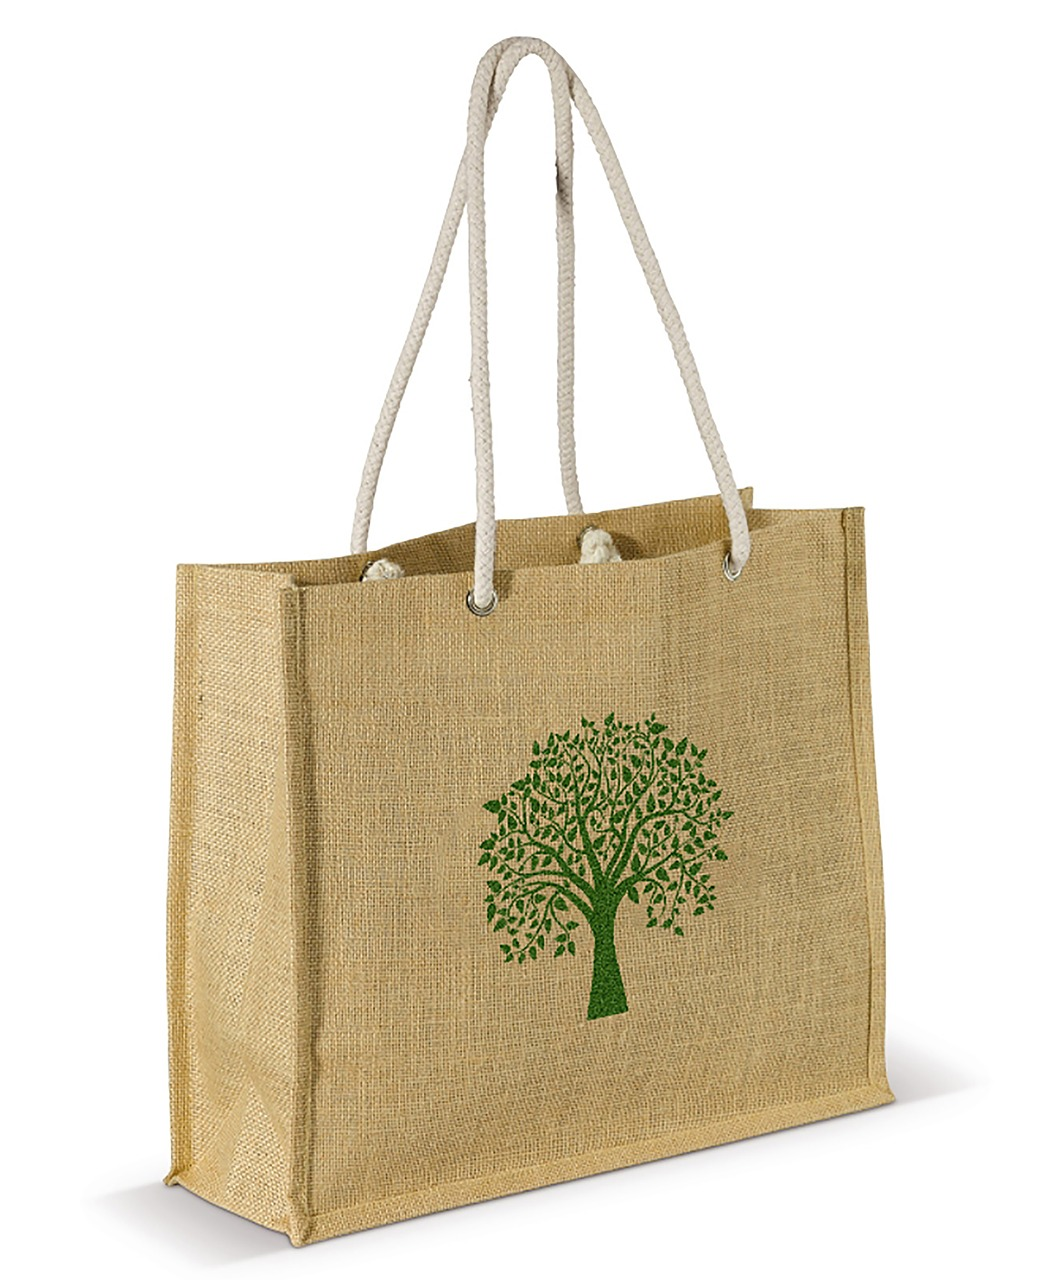
\includegraphics[width=0.9\columnwidth]{../../../FIGURES/divers/doggybag.jpg}
        \end{figure}
    \end{minipage}
\end{frame}

\section{Grandes approches du TAL}

\begin{frame}{Rappel~: le TAL}
    \begin{minipage}{0.35\columnwidth}
        \begin{figure}
            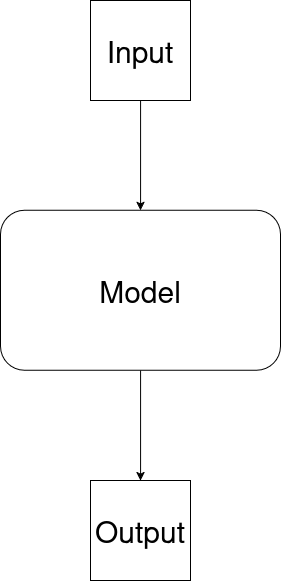
\includegraphics[width=0.7\columnwidth]{../../../FIGURES/découverte_tal/nlp_workflow.png}
        \end{figure}  
    \end{minipage}
    \hfill
    \pause
    \begin{minipage}{0.55\columnwidth}
        \begin{block}{Le TAL}
            \begin{itemize}
                \item Discipline informatique ET linguistique
                \item Traite du texte (écrit ou oral)
                \item langue = un système
            \end{itemize}
        \end{block}
        \vfill
        \pause
        \begin{block}{Trois grandes approches~:}
            \begin{itemize}
                \item Approches à base de règles (linguistique)
                \item Approches statistiques (mathématiques)
                \item Approches neuronales (neurologie)
            \end{itemize}
    \end{block}
    \end{minipage}
\end{frame}

\begin{frame}{Chronologie du TAL}
    \begin{figure}
        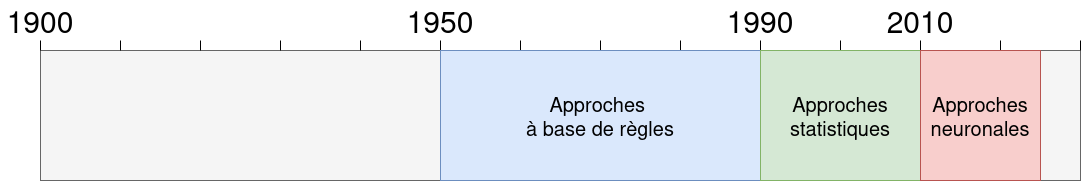
\includegraphics[width=1\columnwidth]{../../../FIGURES/découverte_tal/tal_chronologie.png}
    \end{figure}
    \vfill
    \pause
    \begin{center}
        \Large
        Dans ce cours~: comparaison entre ces trois approches.
    \end{center}
\end{frame}

\begin{frame}{Critères de comparaison}
    \begin{itemize}
        \pause
        \item \textbf{Couverture~:} L'approche gère-t-elle bien les cas ambigus ?
        \pause
        \item \textbf{Précision~:} L'approche identifie-t-elle ce qu'on lui demande ?
        \pause
        \item \textbf{Interprétabilité~:} L'approche est-elle facile à comprendre ?
        \pause
        \item \textbf{Données~:} l'approche nécessite-t-elle beaucoup de données ?
        \pause
        \item \textbf{Ressources~:} l'approche nécessite-t-elle beaucoup de ressources ?
    \end{itemize}
    \vfill
    \pause
    \begin{table}
        \centering
        \renewcommand{\arraystretch}{1.5}  
        \begin{tabular}{|c|c|c|c|c|}
            \hline
            Couverture & Précision & Interprétabilité & Données & Ressources \\
            \hline
                       &           &                  &         &            \\
            \hline
        \end{tabular}
    \end{table}
\end{frame}

\section{Approches à base de règles}

\begin{frame}{Un peu d'histoire~: l'expérience de Georgetown-IBM (1954)}
    % \begin{itemize}
    %     \item 60 phrases russes traduites en anglais
    %     \item 6 règles de grammaire et 250 mots de vocabulaire
    %     \item "la traduction auto. sera résolue d'ici 3 à 5 ans"
    % \end{itemize}
    % \vfill
    \pause
    \begin{figure}
        %\raggedleft
        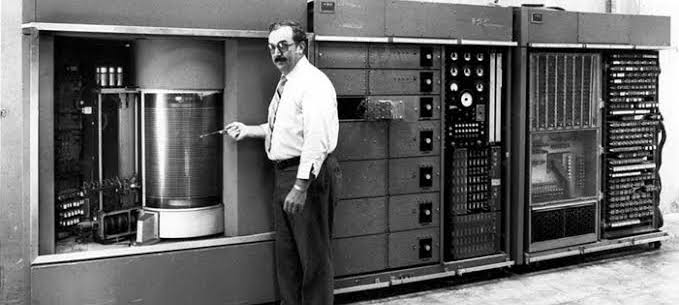
\includegraphics[width=1\columnwidth]{../../../FIGURES/découverte_tal/georgetown_ibm_computer.jpg}
    \end{figure}
\end{frame}

\begin{frame}{Approches à base de règles}
    \pause
    \begin{block}{Propriétés}
        \begin{itemize}
            \item Fonctionne avec des règles
            \item Règle $\Rightarrow$ basée sur connaissances préalable
            \item Règle $\Rightarrow$ suit un schéma logique ("\textit{if... then}", "\textit{if... else}")
        \end{itemize}
    \end{block}
    \vfill
    \pause
    \begin{block}{Types de règles}
        \begin{itemize}
            \item Recherche exacte ("\textit{if token == chat}")
            \item Morphosyntaxe ("\textit{if token == Verb}")
            \item Regex ("\textit{if token == \bs w*ent}")
            \item etc
        \end{itemize}
    \end{block}
\end{frame}

\begin{frame}{Rappel~: le filtre à spams}
    \begin{figure}
        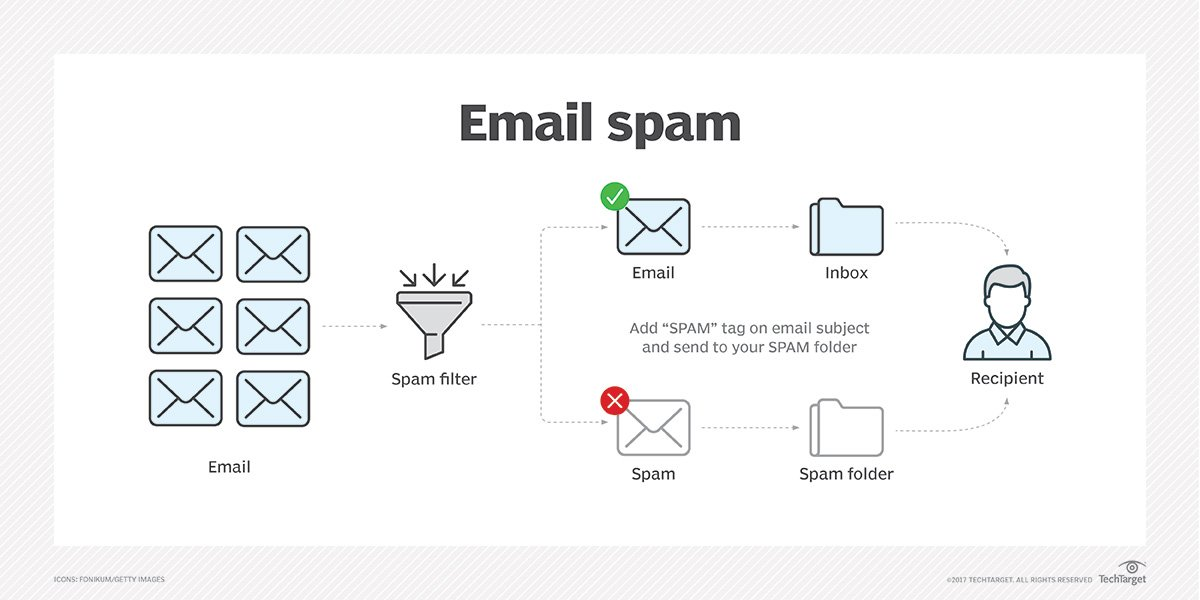
\includegraphics[width=0.8\columnwidth]{../../../FIGURES/découverte_tal/mail_spam_filter.jpg}
        \caption*{Source~: un article d'Andrew Zola\footnote{\url{https://www.techtarget.com/cybersecurity/definition/spam-filter}}}
    \end{figure}
\end{frame}

\begin{frame}{Rappel~: le filtre à spams}
    \begin{block}{Un mail est un spam si...}
        \begin{itemize}
            \item il contient le mot "urgent"
            \item un riche héritier a besoin d'argent
            \item le domaine mail de l'envoyeur est inconnu
            \item il est envoyé 50 fois en 2 heures
            \item etc
        \end{itemize}
    \end{block}
    \vfill
    \pause
    \begin{table}
        \centering
        \renewcommand{\arraystretch}{1.5}  
        \begin{tabular}{|c|c|c|c|c|}
            \hline
            Couverture & Précision & Interprétabilité & Données & Ressources \\
            \hline
            ?          & ?         & ?                & ?       & ?          \\
            \hline
        \end{tabular}
    \end{table}
\end{frame}

\begin{frame}{Rappel~: le filtre à spams}
    \begin{itemize}
        \item \textbf{Couverture~:} un spam peut ne pas respecter les règles énoncées
        \begin{itemize}
            \item il y aura toujours des mails échappant à ces règles
        \end{itemize}
        \vfill
        \item \textbf{Précision~:} tous les mails identifiés comme spams respectent les règles énoncées
        \begin{itemize}
            \item si un mail respecte toutes ces règles, il s'agit probablement d'un spam
        \end{itemize}
        \vfill
        \item \textbf{Interprétabilité~:} on comprend pourquoi un mail est identifié comme spam
        \begin{itemize}
            \item on a fixé les règles nous-même
        \end{itemize}
        \vfill
        \item \textbf{Données~:} aucune données utilisées
        \begin{itemize}
            \item nous n'avons pas besoin de données pour créer ces règles
        \end{itemize}
        \vfill
        \item \textbf{Ressources~:} très peu de ressources sollicitées
        \begin{itemize}
            \item les règles sont des conditions, elles se calculent vite
        \end{itemize}
    \end{itemize}
\end{frame}

\begin{frame}{Rappel~: le filtre à spams}
    \begin{block}{Un mail est un spam si...}
        \begin{itemize}
            \item il contient le mot "urgent"
            \item un riche héritier a besoin d'argent
            \item le domaine mail de l'envoyeur est inconnu
            \item il est envoyé 50 fois en 2 heures
            \item etc
        \end{itemize}
    \end{block}
    \vfill
    \begin{table}
        \centering
        \renewcommand{\arraystretch}{1.5}  
        \begin{tabular}{|c|c|c|c|c|}
            \hline
            Couverture & Précision & Interprétabilité & Données & Ressources \\
            \hline
            $-$        & $++$      & $+++$            & $---$   & $---$      \\
            \hline
        \end{tabular}
    \end{table}
\end{frame}

\begin{exoframe}
    \begin{center}
        \Large
        Quelles règles pour identifier des chats ?
    \end{center}
\end{exoframe}

\begin{frame}{Des règles pour identifier des chats}
    \begin{minipage}{0.4\columnwidth}
        \begin{block}{Un chat se caractérise par...}
            \begin{itemize}
                \item des poils
                \item 4 pattes
                \item 1 tête
                \item etc
            \end{itemize}
        \end{block}
    \end{minipage}
    \hfill
    \pause
    \begin{minipage}{0.5\columnwidth}
        \begin{figure}
            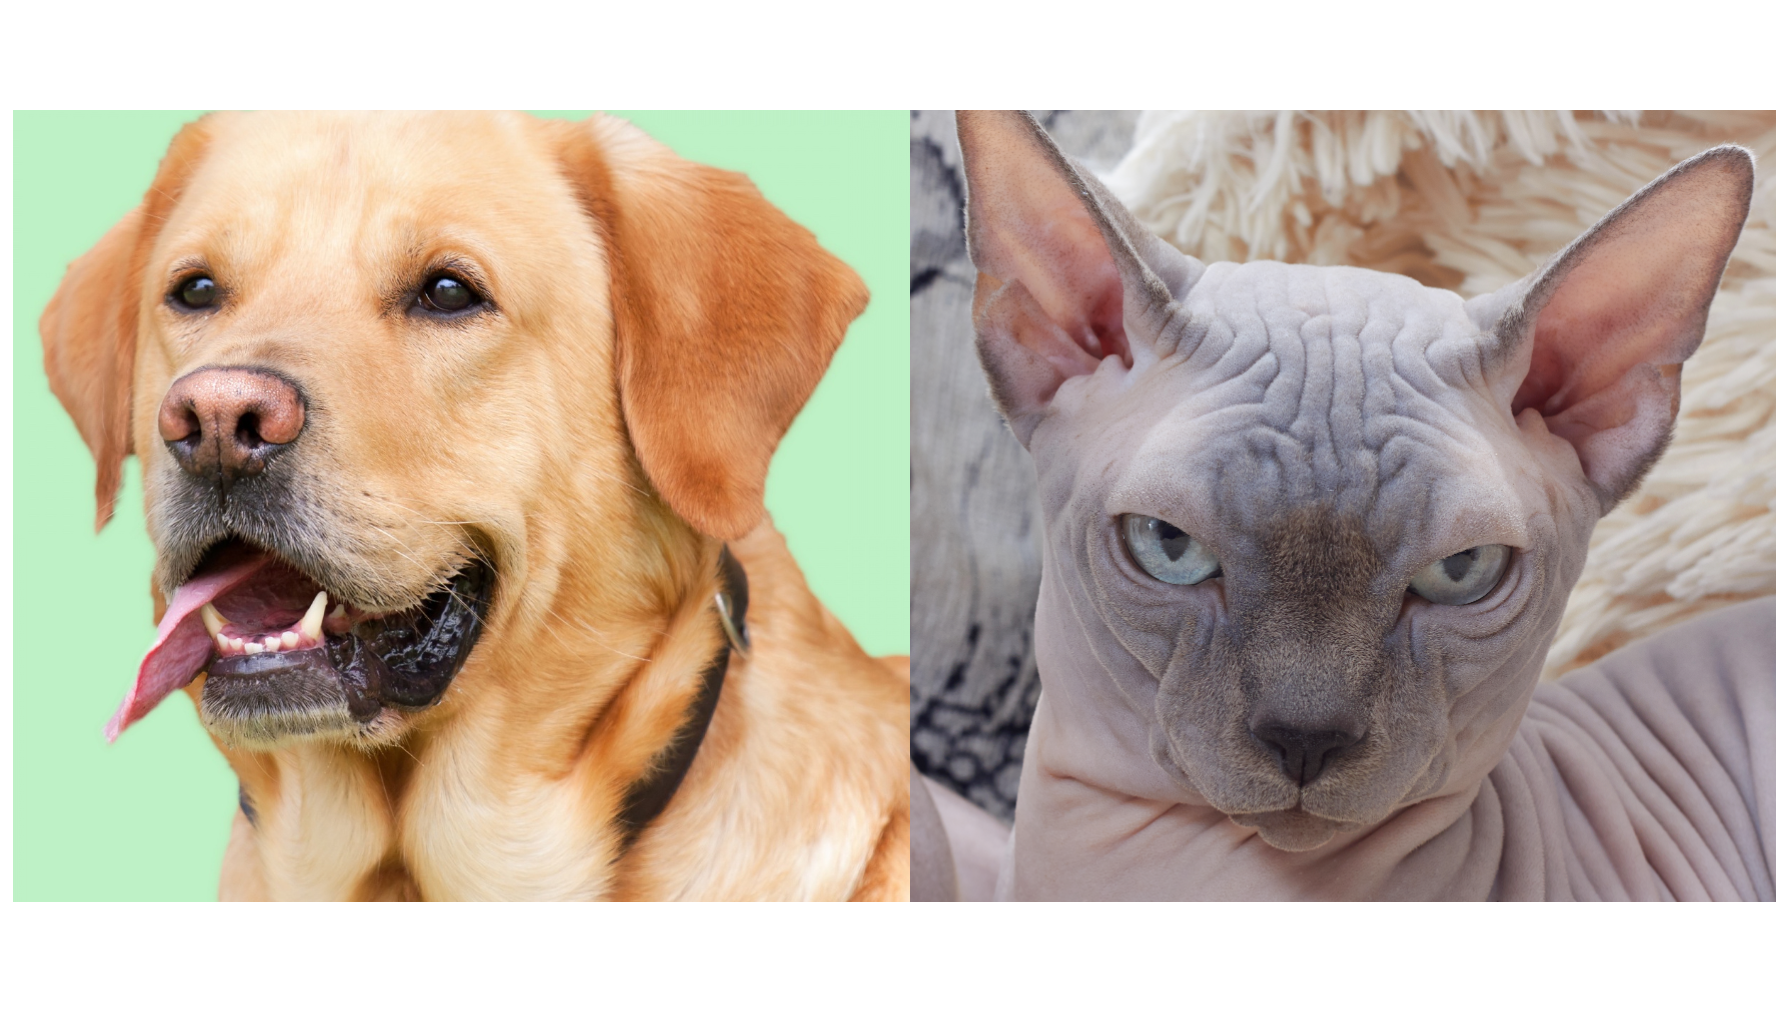
\includegraphics[width=1\columnwidth]{../../../FIGURES/découverte_tal/chat_chien.png}
        \end{figure}
    \end{minipage}
    \vfill
    \pause
    \begin{center}
        \Large
        Différents types d'erreurs possibles !
    \end{center}
\end{frame}
 % \begin{itemize}
    %     \item Première traduction probabiliste par IBM
    %     \item Traduction de l'anglais vers le français
    %     \item Limite~: les données
    % \end{itemize}
    % \vfill
\section{Approches statistiques}

\begin{frame}{Un peu d'histoire~: l'avènement des statistiques (1990)}
    % \begin{itemize}
    %     \item Première traduction probabiliste par IBM
    %     \item Traduction de l'anglais vers le français
    %     \item Limite~: les données
    % \end{itemize}
    % \vfill
    \pause
    \begin{figure}
        %\raggedleft
        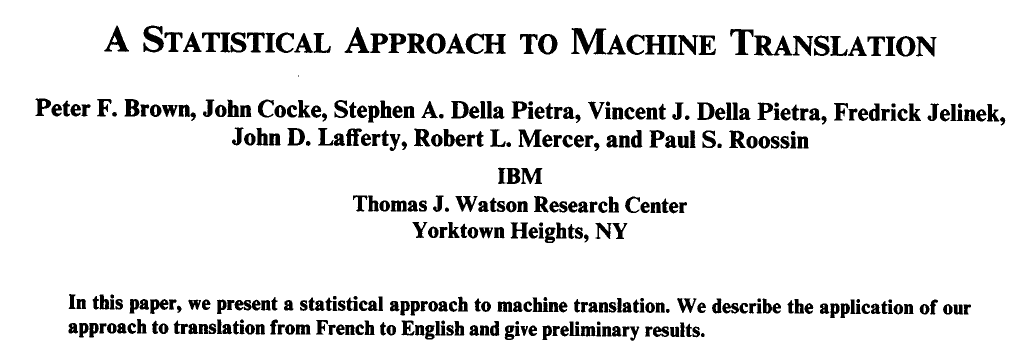
\includegraphics[width=1\columnwidth]{../../../FIGURES/découverte_tal/IBM_statistical_translation.png}
    \end{figure}
\end{frame}

\begin{frame}{Approches statistiques}
    \pause
    \begin{block}{Idée de départ}
        \begin{itemize}
            \item Langue = beaucoup de règles implicites
            \item Au lieu de formuler ces règles, on peut identifier des paternes
            \item Paterne~: quelque chose de régulier et de fréquent
        \end{itemize}
    \end{block}
    \vfill
    \pause
    \begin{block}{Exemple de paterne}
        \begin{itemize}
            \item Entités nommées
            \item Structures morphosyntaxiques
            \item Mails correspondant à des spams
        \end{itemize}
    \end{block}
\end{frame}

%TODO année pro:
%améliorer ce cours:
%graphes N dimensions avec N = taille vecteur
%on réduit tt à 2 dimensions pour que ça soit lisible => méthodes ?
%exemple du livre : quand on ouvre un livre, on a plein de dimensions
    % (une page = une dimension)
    % chaque vecteur est quelque part entre ces dimensions
    % quand on ferme le livre, tout s'empile sur 2 dimensions
% parler de linéaire vs non linéaire 
    % linéaire: c'est une droite.
    % non linéaire : on fait varier la forme

\begin{frame}{Avec des chats...}
    \pause
    \begin{block}{Pas de règle, mais des hypothèses}
        \begin{itemize}
            \item Tous les chats se ressemblent
            \item En tant qu'humain, on peut identifier des chats
            \item Pas besoin de lister des règles pour identifier des chats
        \end{itemize}
    \end{block}
    \vfill
    \pause
    \begin{center}
        \Large
        On laisse le modèle trier les images de chat. \\
        Performance du modèle~: dépendant des données !
    \end{center}
\end{frame}

\begin{frame}{Étape OBLIGATOIRE~: la vectorisation}
    \begin{figure}
        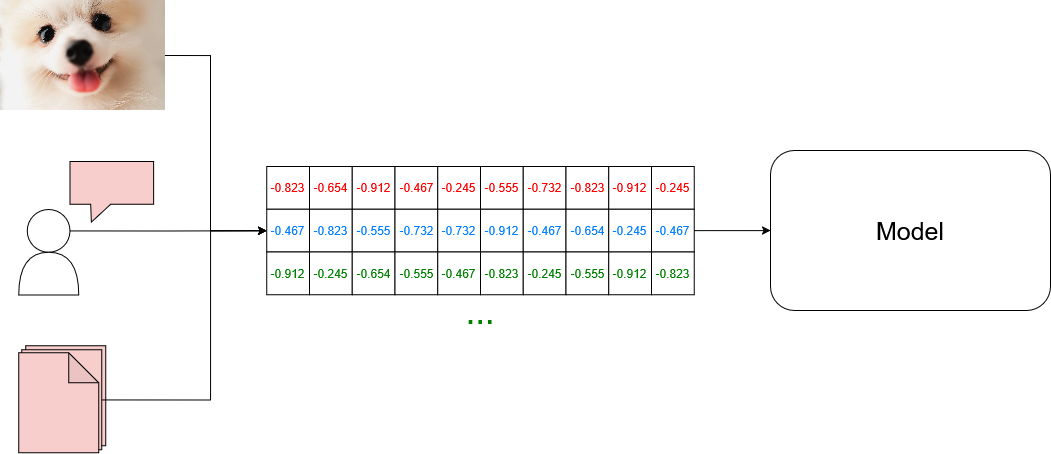
\includegraphics[width=0.8\columnwidth]{../../../FIGURES/découverte_tal/vectorization.png}
    \end{figure}
    \vfill
    \pause
    \begin{center}
        \Large
        Chaque donnée a son vecteur, qui peut être placé sur un graphe \\
        de dimension $N$ ($N$ = taille des vecteurs).
    \end{center}
\end{frame}

\begin{frame}{Rappel~: les différentes méthodes de vectorisation}
    \begin{figure}
        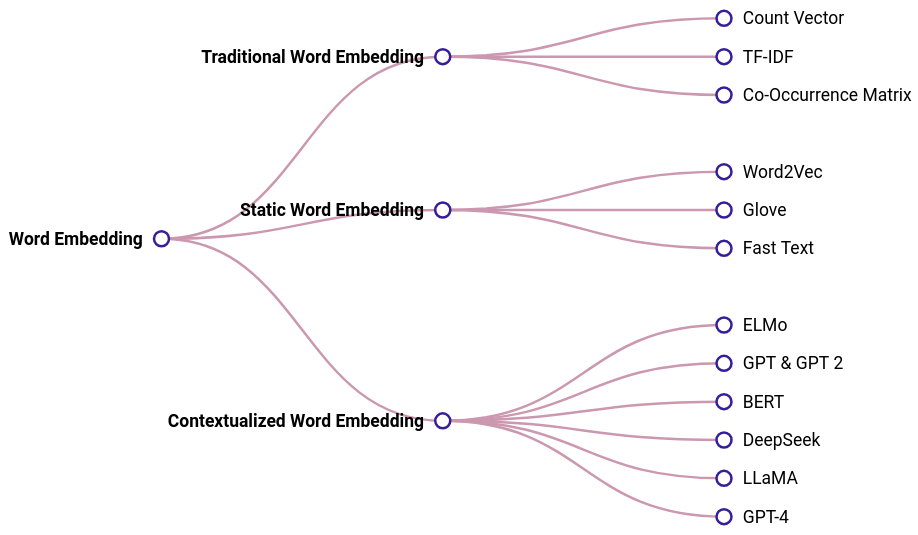
\includegraphics[width=0.7\columnwidth]{../../../FIGURES/découverte_tal/vectorization_processes.png}
        \caption*{Source~: Hesam Sheikh Hassani\footnote{\url{https://huggingface.co/hesamation}}}
    \end{figure}
\end{frame}

% \begin{frame}{Exemple~: les SVM}
%     \begin{figure}
%         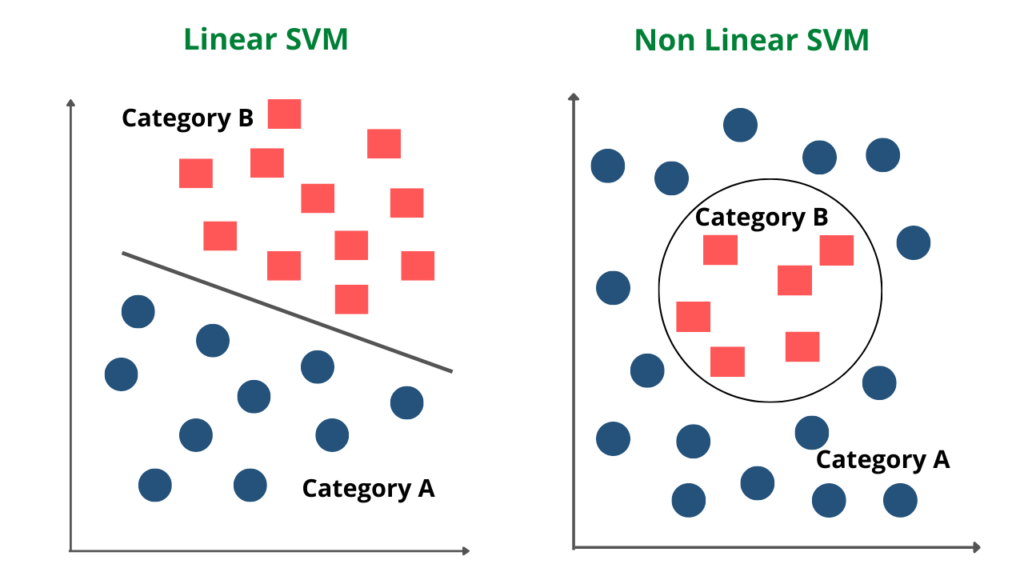
\includegraphics[width=0.7\columnwidth]{../../../FIGURES/découverte_tal/svm_example.png}
%         \caption*{Source~: Naem Azam Chowdhury sur Medium\footnote{\url{https://naemazam.medium.com}}}
%     \end{figure}
% \end{frame}

\begin{frame}{Exemple~: les SVM}
    \begin{figure}
        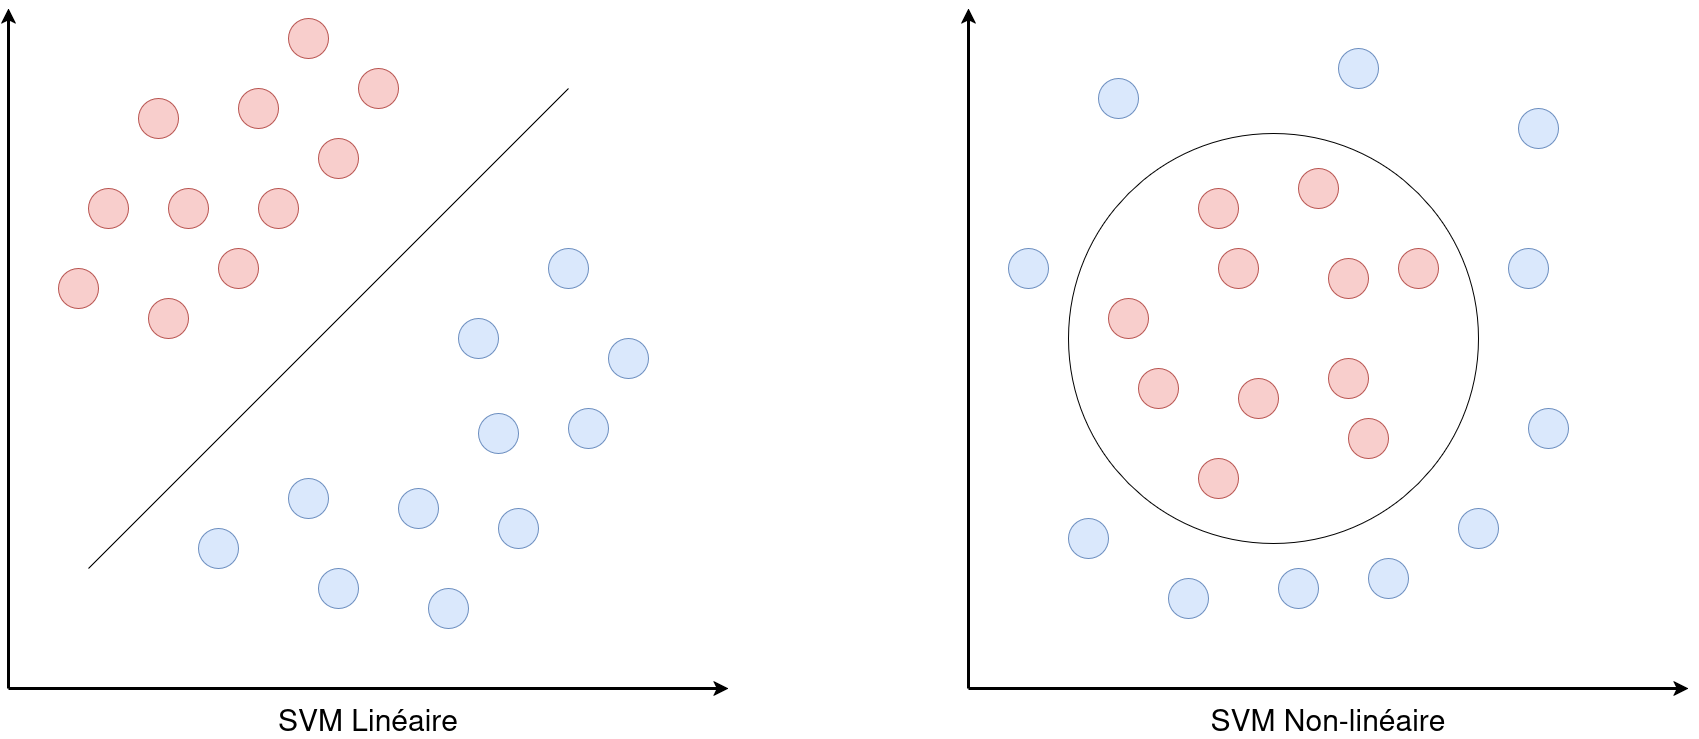
\includegraphics[width=1\columnwidth]{../../../FIGURES/découverte_tal/statistical_classif_graph.png}
    \end{figure}
\end{frame}

\begin{frame}{Exemple~: les SVM}
    \begin{block}{Comment ça marche ?}
        \begin{itemize}
            \item On vectorise des données
            \begin{itemize}
                \item Ronds rouges~: les mails correspondant à des chats
                \item Ronds bleus~: les mails ne correspondant pas à des chats
            \end{itemize}
            \vspace{10pt}
            \item On entraîne une approche sur ces données
            \begin{itemize}
                \item On choisi une approche et on l'entraîne sur les données
                \item Cela détermine la position de la ligne (et sa forme si approche non-linéaire)
            \end{itemize}
        \end{itemize}
    \end{block}
    \vfill
    \only<1>{\color{white}
        \begin{center}
            \Large
            Vectorisation~: on détermine la position des points. \\
            Entraînement~: on cherche la ligne séparant ces points.
        \end{center}
    }
    \only<2>{
        \begin{center}
            \Large
            Vectorisation~: on détermine la position des points. \\
            Entraînement~: on cherche la ligne séparant ces points.
        \end{center}
    }
    \only<3>{
        \begin{table}
            \centering
            \renewcommand{\arraystretch}{1.5}  
            \begin{tabular}{|c|c|c|c|c|}
                \hline
                Couverture & Précision & Interprétabilité & Données & Ressources \\
                \hline
                ?          & ?         & ?                & ?       & ?          \\
                \hline
            \end{tabular}
        \end{table}
    }
    \only<4>{
        \begin{table}
            \centering
            \renewcommand{\arraystretch}{1.5}  
            \begin{tabular}{|c|c|c|c|c|}
                \hline
                Couverture & Précision & Interprétabilité & Données & Ressources \\
                \hline
                $++$       & $+$      & $-$              & $++$     & $+$        \\
                \hline
            \end{tabular}
        \end{table}
    }
\end{frame}

\section{Approches neuronales}

\begin{frame}{Un peu d'histoire~: les réseaux de neurones}
    % \begin{itemize}
    %     \item Approches statistiques $\Rightarrow$ représentations statiques
    %     \item Approches neuronales $\Rightarrow$ représentations contextuelles
    %     \item Limite~: beaucou plus de données !
    % \end{itemize}
    % \vfill
    \pause
    \begin{figure}
        % \raggedleft
        
\includegraphics[width=1\columnwidth]{../../../FIGURES/découverte_tal/neural_network_paper.png}
    \end{figure}
\end{frame}

\begin{frame}{Approches neuronales}
    \pause
    \begin{block}{Les approches neuronales sont des approches statistiques}
        \begin{itemize}
            \item On ne cherche pas à expliciter des règles
            \item On cherche plutôt à identifier des paternes
            \item Le modèle va s'entraîner par itération
        \end{itemize}
    \end{block}
    \vfill
    \pause
    \begin{block}{À chaque itération, le modèle...}
        \begin{itemize}
            \item Fait une prédiction (prochain mot, label, etc)
            \item Regarde si sa prédiction est correcte (mesure de performance)
            \item Modifie les représentations (vecteurs) pour ajuster le tir
            \item Recommence l'opération des milliers / millions de fois
        \end{itemize}
    \end{block}
\end{frame}

\begin{frame}{Comment fonctionne un réseau de neurones ?}
    %https://www.youtube.com/watch?v=SV2huMdNs9c
    \begin{center}
        \Large
        Question~: Devrais-je aller au parc avec mes amis ?
    \end{center}
    \vfill
    \begin{block}{Critères}
        \begin{itemize}
            \item Fait-il beau ? 
            \item Mes amis sont-ils disponibles ?
            \item Ai-je terminé mes devoirs ?
        \end{itemize}
    \end{block}
    \vfill
    \begin{block}{Réponses possibles}
        \begin{itemize}
            \item Oui ou non
        \end{itemize}
    \end{block}
    \vfill
    \begin{block}{Algorithme}
        \begin{itemize}
            \item Si deux critères sont validés, j'y vais
        \end{itemize}
    \end{block}
\end{frame}

\begin{frame}{Comment fonctionne un réseau de neurones ?}
    \begin{figure}
        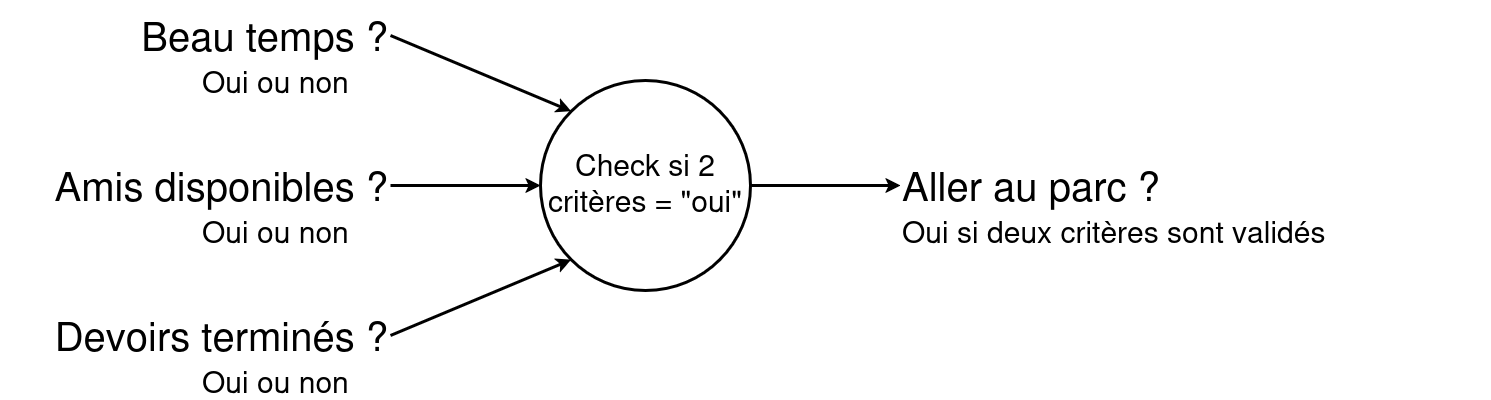
\includegraphics[width=1\columnwidth]{../../../FIGURES/découverte_tal/neural_network/tuto_neural_network_1.png}
    \end{figure}
    \vfill
    \begin{center}
        \Large
        On schématise les critères, l'algorithme et la sortie.
    \end{center}
\end{frame}

\begin{frame}{Comment fonctionne un réseau de neurones ?}
    \begin{figure}
        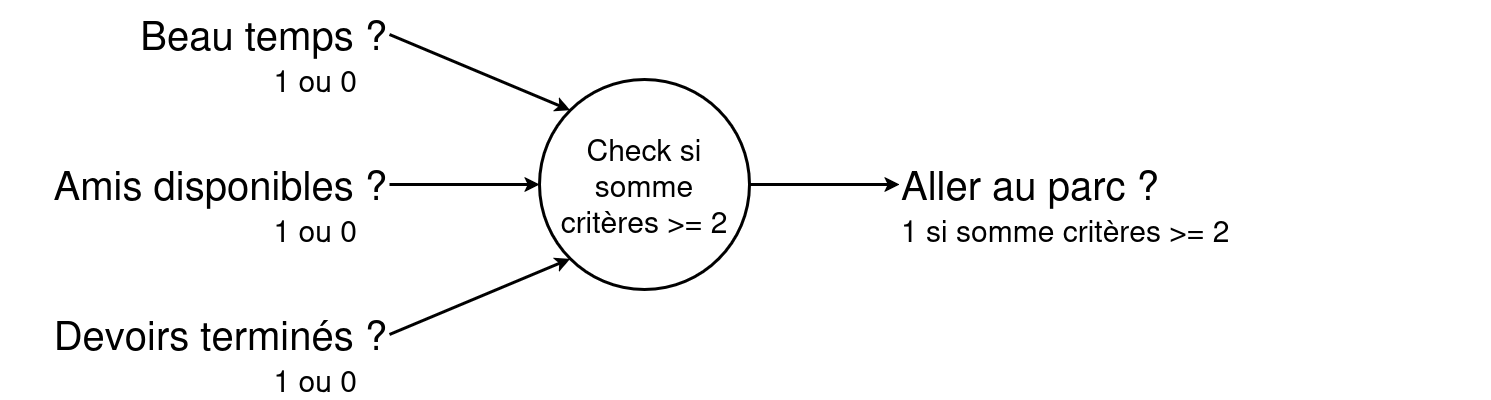
\includegraphics[width=1\columnwidth]{../../../FIGURES/découverte_tal/neural_network/tuto_neural_network_2.png}
    \end{figure}
    \vfill
    \begin{center}
        \Large
        On remplace "oui" par 1 et "non" par 0.
    \end{center}
\end{frame}

\begin{frame}{Comment fonctionne un réseau de neurones ?}
    \begin{figure}
        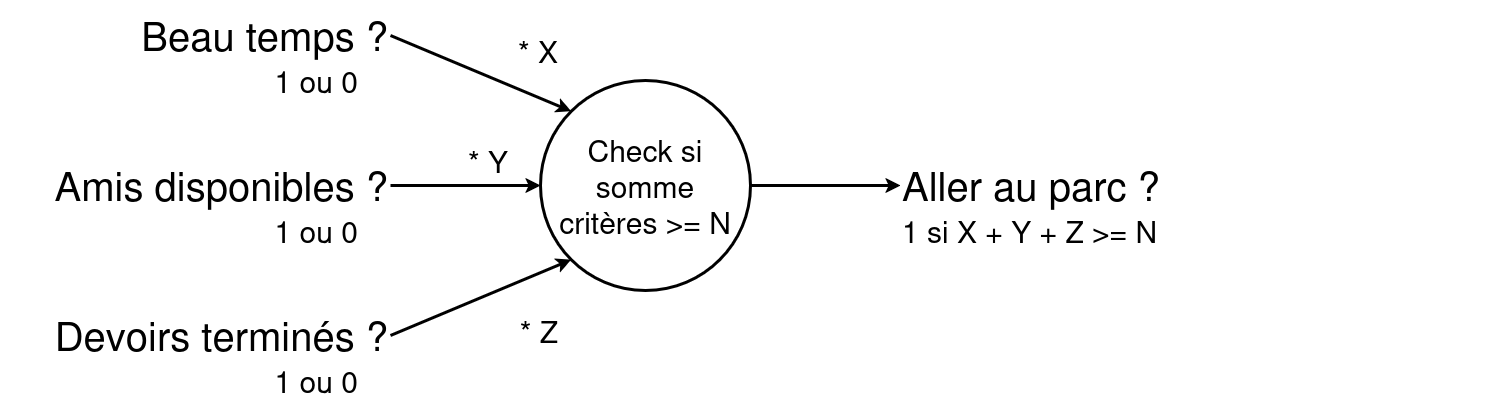
\includegraphics[width=1\columnwidth]{../../../FIGURES/découverte_tal/neural_network/tuto_neural_network_3.png}
    \end{figure}
    \vfill
    \begin{center}
        \Large
        On ajoute un poids pour chaque critères.
    \end{center}
\end{frame}

\begin{frame}{Comment fonctionne un réseau de neurones ?}
    \begin{figure}
        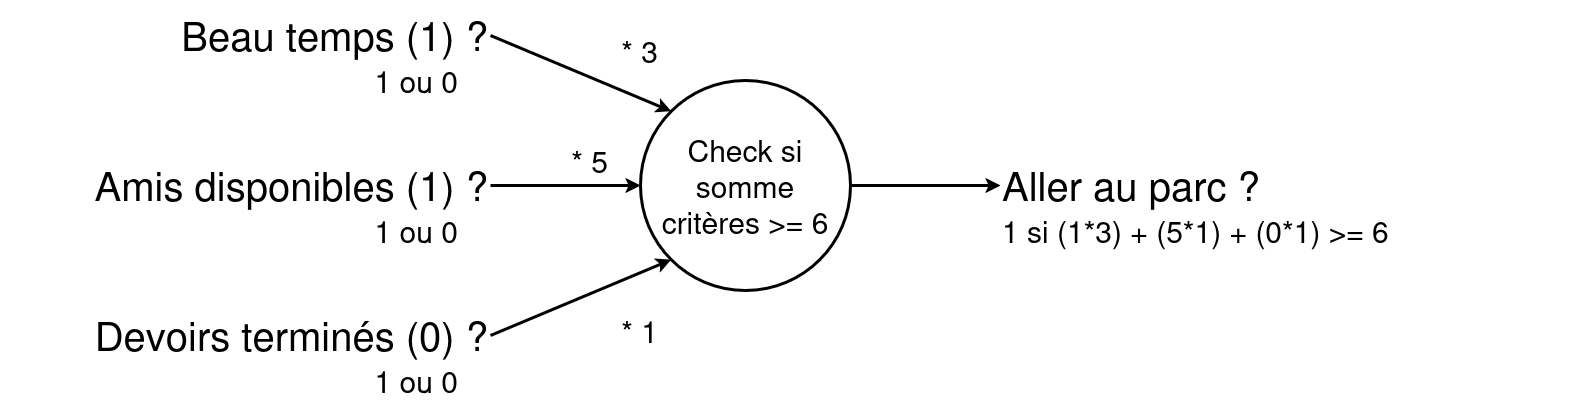
\includegraphics[width=1\columnwidth]{../../../FIGURES/découverte_tal/neural_network/tuto_neural_network_4.png}
    \end{figure}
    \vfill
    \begin{center}
        \Large
        Exemple en remplaçant les variables par de vraies valeurs.
    \end{center}
\end{frame}

\begin{frame}{Comment fonctionne un réseau de neurones ?}
    \begin{minipage}{0.45\columnwidth}
        Source~: \\ \url{https://www.youtube.com/watch?v=SV2huMdNs9c}
    \end{minipage}
    \hfill
    \begin{minipage}{0.45\columnwidth}
        \begin{figure}
            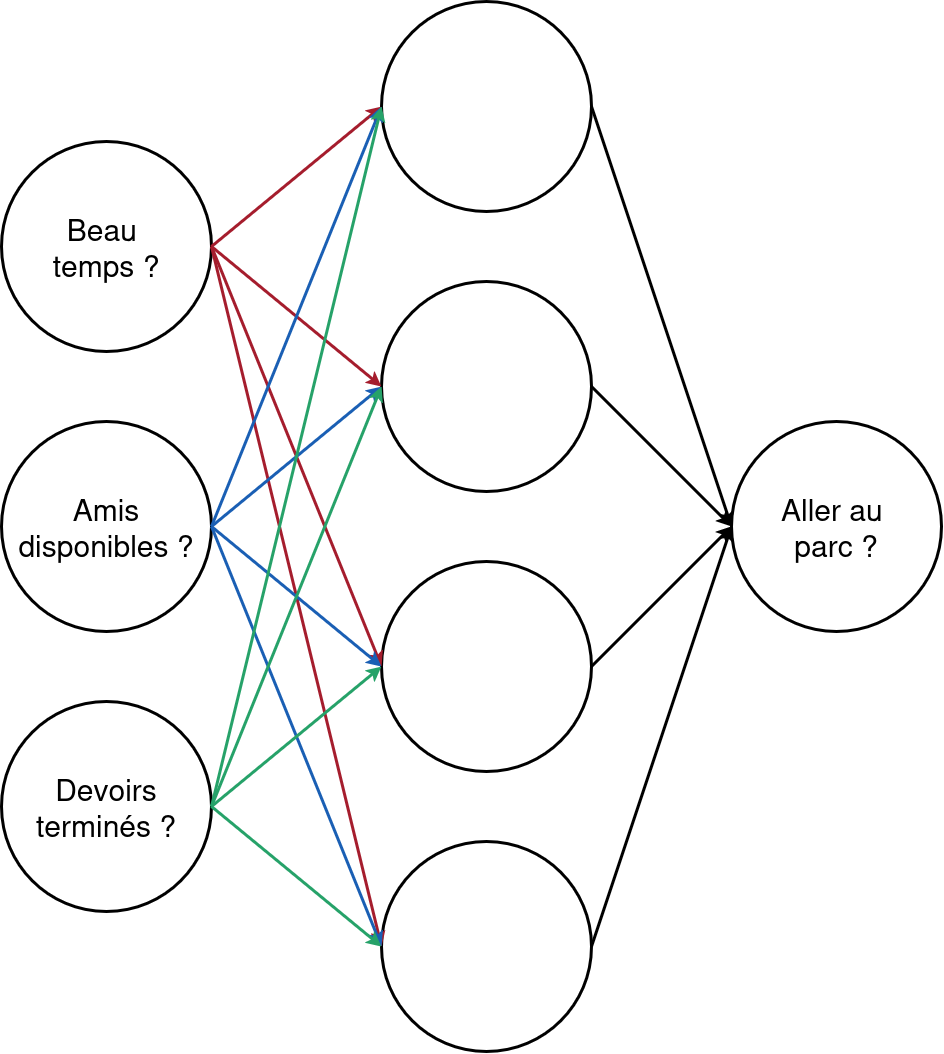
\includegraphics[width=1\columnwidth]{../../../FIGURES/découverte_tal/neural_network/tuto_neural_network_5.png}
    \end{figure}
    \end{minipage}
\end{frame}

\begin{frame}{Ce qu'il se passe dans le graphe...}
    \begin{figure}
        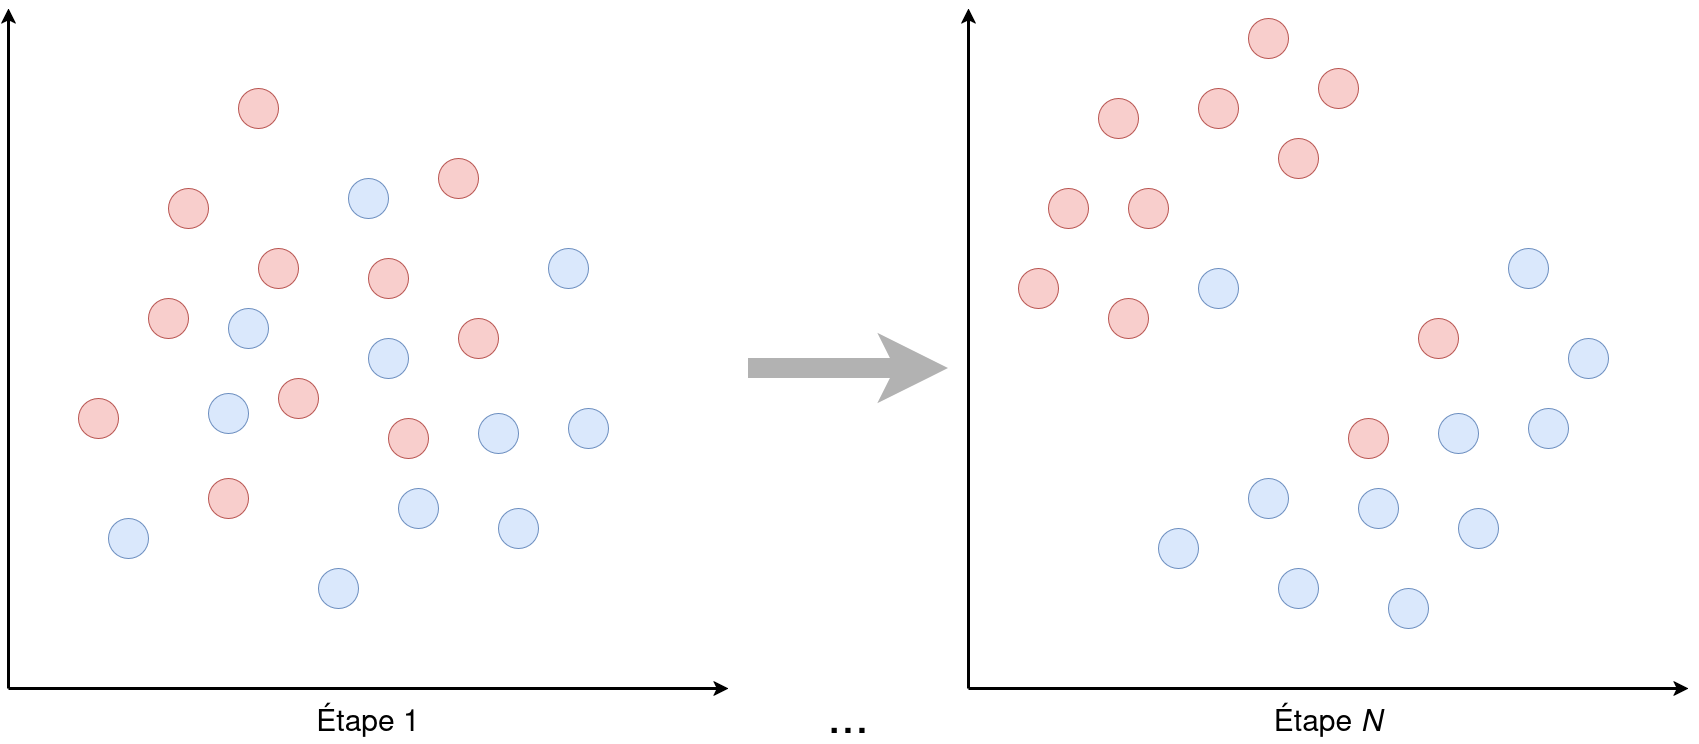
\includegraphics[width=1\columnwidth]{../../../FIGURES/découverte_tal/neural_classsif_graph.png}
    \end{figure}
\end{frame}

\begin{frame}{Ce qu'il se passe dans le graphe...}
    \begin{block}{Comment ça marche ?}
        \begin{itemize}
            \item On vectorise des données
            \begin{itemize}
                \item Ronds rouges~: les mails correspondant à des chats
                \item Ronds bleus~: les mails ne correspondant pas à des chats
            \end{itemize}
            \vspace{10pt}
            \item On entraîne un réseau de neurones sur ces données
            \begin{itemize}
                \item À chaque étape, le modèle fait varier les représentations
                \item Il vérifie ensuite s'il classifie mieux les chats avec ces représentations
            \end{itemize}
        \end{itemize}
    \end{block}
    \vfill
    \only<2>{
        \begin{table}
            \centering
            \renewcommand{\arraystretch}{1.5}  
            \begin{tabular}{|c|c|c|c|c|}
                \hline
                Couverture & Précision & Interprétabilité & Données & Ressources \\
                \hline
                ?          & ?         & ?                & ?       & ?          \\
                \hline
            \end{tabular}
        \end{table}
    }
    \only<3>{
        \begin{table}
            \centering
            \renewcommand{\arraystretch}{1.5}  
            \begin{tabular}{|c|c|c|c|c|}
                \hline
                Couverture & Précision & Interprétabilité & Données & Ressources \\
                \hline
                $+++$      & $++$      & $---$            & $+++$   & $+++$      \\
                \hline
            \end{tabular}
        \end{table}
    }
\end{frame}

\begin{frame}{Les réseaux de neurones sont légions}
    \begin{minipage}{0.45\columnwidth}
        \begin{figure}
            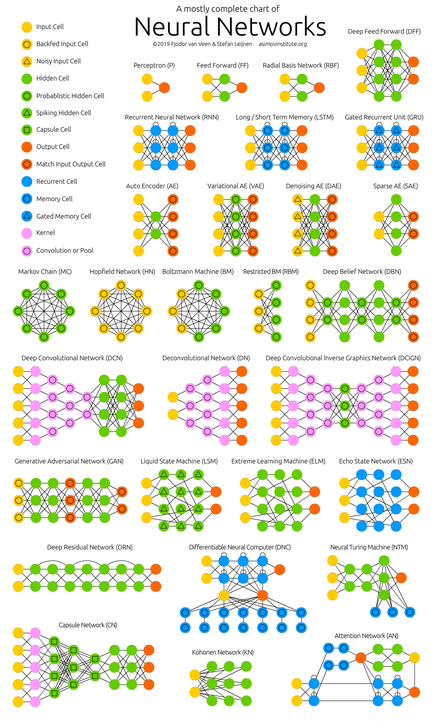
\includegraphics[width=0.7\columnwidth]{../../../FIGURES/découverte_tal/neural_network_zoo.png}
        \end{figure}
    \end{minipage}
    \hfill
    \begin{minipage}{0.45\columnwidth}
        Source~: \\ \url{https://www.asimovinstitute.org/neural-network-zoo/}
    \end{minipage}
\end{frame}

% \begin{exoframe}
%     \begin{center}
%         \Large
%         Quand appliquer une approche statistique ?
%     \end{center}
%     \vfill
%     \pause
%     \begin{itemize} \color{white}
%         \item Quantité importante de données à traiter
%         \item Les données / classes sont ambigues 
%     \end{itemize}
% \end{exoframe}

\begin{frame}{Doggy bag}
    \begin{minipage}{0.45\columnwidth}
        \begin{block}{Approches à base de règles}
            \begin{itemize}
                \item Basées sur la linguistique 
                \item Très interprétables
            \end{itemize}
        \end{block}
        \vfill
        \begin{block}{Approches statistiques}
            \begin{itemize}
                \item Paterne~: régulier et fréquent
                \item Vectorisation des données
            \end{itemize}
        \end{block}
        \vfill
        \begin{block}{Approches neuronales}
            \begin{itemize}
                \item BEAUCOUP de données
                \item BEAUCOUP de calculs
            \end{itemize}
        \end{block}
    \end{minipage}
    \hfill
    \begin{minipage}{0.45\columnwidth}
        \begin{figure}
            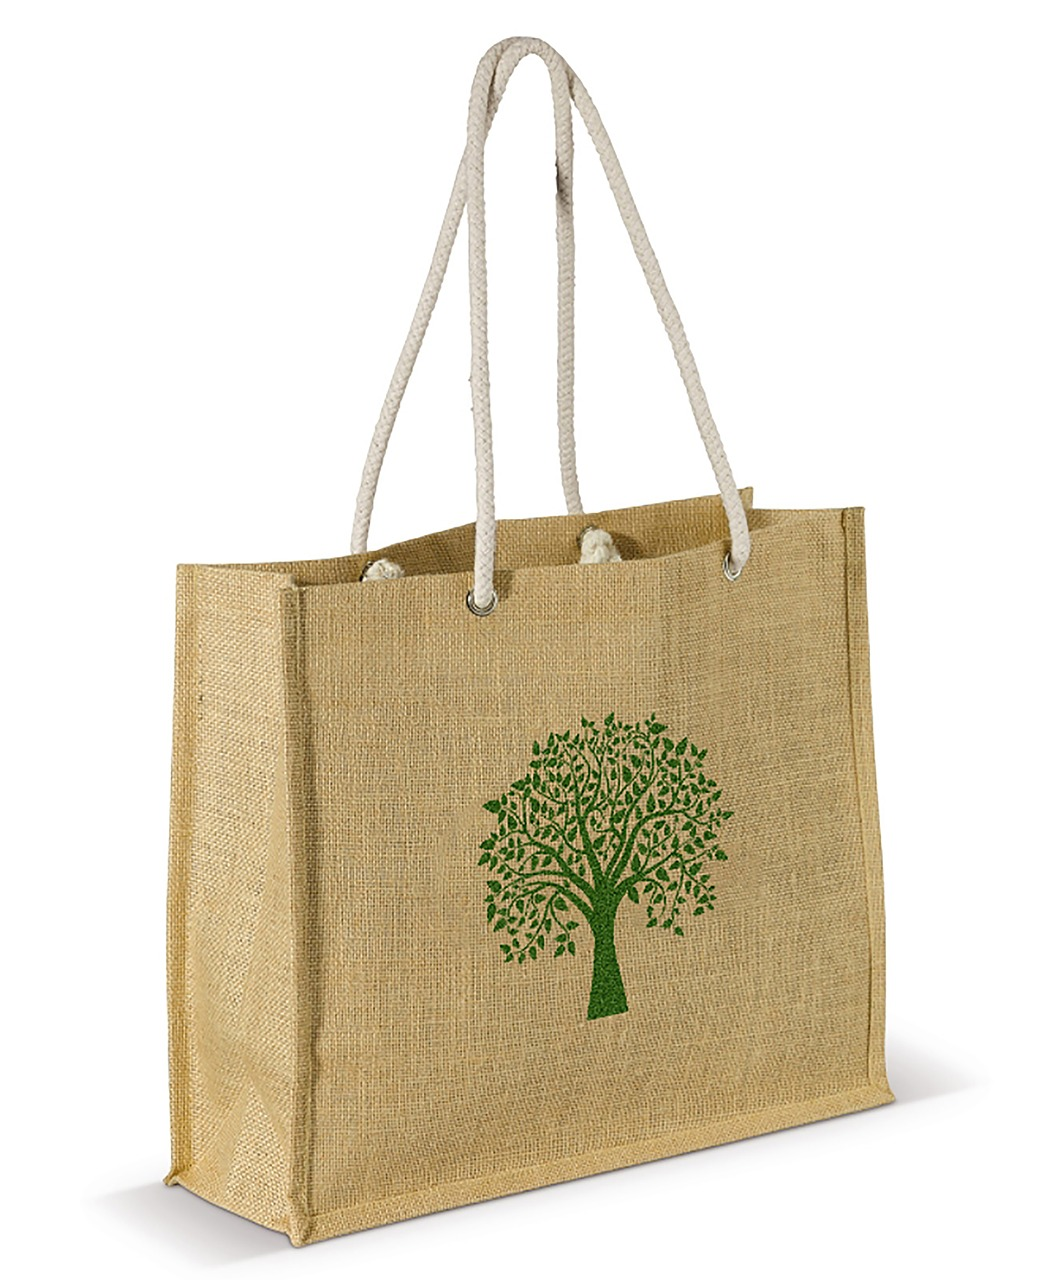
\includegraphics[width=0.9\columnwidth]{../../../FIGURES/divers/doggybag.jpg}
        \end{figure}
    \end{minipage}
\end{frame}

\end{document}

